%% Use this line for the final version of your report
%\documentclass[final,English]{include/RaM/RaM-MScReport}

%% Use this line for the draft versions of your report, it enables rro/notes/line numbers/date in footer
\documentclass[lineno,english]{include/RaM/RaM-MScReport}

\settitle{Project Plan}
\setauthor{Wolfgang Baumgartner}
\setsubject{project plan for the production phase}
\setkeywords{project plan, ideas, time management}
%-------------------------------------------------------------------------------------------------
% This settings.tex contains settings required for *all* documents (reports, presentations, etc)
% Project or Report specific settings should go to their own settings files (eg CE/settings.tex)
% This file is included after the class definition and before project and report specific settings 
%-------------------------------------------------------------------------------------------------

%--------Useful packages (required by the example files, turn off if you do not use them)-------
\usepackage{babel}					% Add language specific support
%\usepackage{makeidx}				% Index support
%\usepackage[totoc,justific=RaggedRight]{idxlayout}	% Make last page of index balanced and add index to toc
\usepackage{caption}				% Provides means to style captions
%\usepackage{subcaption}				% Provides support for (sub)figures and (sub)tables
%\usepackage{float}					% Improved interface for floating objects (eg figures, tables, ...)
\usepackage{enumitem}				% Add styling support to (enumerate) environments
\usepackage{listings}				% Allows (external) source files to be shown in a syntax highlighted way
%\usepackage{amsmath}				% Provides miscellaneous enhancements for documents containing formulas
\usepackage{datetime}				% Provides commands for displaying the current time
%\usepackage{etoolbox}				% Provides \AtBeginEnvironment command
\usepackage{eurosym}				% Defines \euro command to display euro symbols
%\usepackage{appendix}				% Makes it possible to modify appendix numbering
%\usepackage{longtable}				% Allows tables to span multiple pages
%\usepackage{units}					% Shows units (eg m/s) in a nice way
%\usepackage{ctable}				% Provides \ctable command for the typesetting of table and figure floats
%\usepackage{ccaption}				% Support continuation captions (eg multi-page tables)
%\usepackage{verbatim}				% Adds verbatim environment, in which texts are exactly copied to the output
%\usepackage{pdfpages}				% Include PDF pages/documents in the current document
\usepackage{include/files/requirements}

\iffinalversion
	\usepackage[final]{include/files/notes}% Add note commands, [final] removes all notes from the document
	\usepackage[final]{include/files/rro}  % Add Rich Report Outline support, [final] removes all RRO output from document
\else
	\usepackage{include/files/notes}       % Add note commands
	\usepackage{include/files/rro}         % Add Rich Report Outline support
\fi

% Add wrongly (or unknown) hyphened words here (space separated and - at possible hyphenation positions):
%\hyphenation{}

%% Spacing possibilities for captions are available as well
% See captions.pdf for all options!
\captionsetup{font=small,labelfont=bf}

%% Center all figures by default
%% http://tex.stackexchange.com/questions/2651/should-i-use-center-or-centering-for-figures-and-tables
\makeatletter
\g@addto@macro\@floatboxreset\centering
\makeatother

%% Make use small font size in verbatim environment
% Note: AtBeginEnvironment is provided by etoolbox package
%\AtBeginEnvironment{verbatim}{\small}

%% Include verbatim in the subfigure env
% From: subfig.pdf, section 4.4
% <Uncomment if verbatim is required in subfloat>:
%\makeatletter
%\newbox\sf@box
%\let\orig@subfloat\subfloat
%\renewenvironment{subfloat}[2][]%
%{ \def\sf@one{#1}%
%  \def\sf@two{#2}%
%  \setbox\sf@box\hbox
%  \bgroup}%
%{ \egroup
%  \ifx\@empty\sf@two\@empty\relax
%    \def\sf@two{\@empty}
%  \fi
%  \ifx\@empty\sf@one\@empty\relax
%    \orig@subfloat[\sf@two]{\box\sf@box}%
%  \else
%    \orig@subfloat[\sf@one][\sf@two]{\box\sf@box}%
%  \fi}
%\makeatother
%% Uncomment till here
  
%% Automatically provide H option for floats
% Requires float package
% \floatplacement{figure}{H} 
% \floatplacement{table}{H} 

%% abbreviation making
\newcommand{\abbr}[1]{(\textit{#1})}

%%lstlisting settings
\lstset{	%aboveskip=20pt,%
		numbers=none, %no line numbers
%		numbers=left, %show line numbers
		numberstyle=\tiny,%
		frame=single,%
		frameround={t}{t}{t}{t},%
		numbersep=5pt,%
%		language=C,% (default) code language in the document
		captionpos=b,%
		xleftmargin=2em,
		framexleftmargin=1.5em,
		xrightmargin=2em,
		framexrightmargin=1.5em,
		morecomment=[s][\itshape]{<}{>}, %also define <> as comment
		morecomment=[s][\itshape]{[}{]} %also define [] as comment
}

%lstinline with empty language definition
\lstdefinelanguage{empty}{}
\newcommand{\mylstinline}[1]{{\lstinline[language=empty]{#1}}}

% Default value of top separator (empty space) of lists
\setlist{topsep=4pt}

%% Don't show warnings like: ``PDF inclusion: found PDF version <1.x>, but at most version <1.4> allowed
% Uncomment if you experience these kind of warnings 
%\ifpdf
%	\pdfminorversion=6 
%\fi


\begin{document}
% Numbered roman style

\makerro				% Build RichReportOutline.rro file

\frontmatter

% Use \maketitle or the available PDF when it is released (for student reports)
\maketitle

% Enter the name of the official RaM title page PDF between the brackets
% ! This method disables the option of using EPS files in your report.
% ! If EPS images are required, use LaTeX source instead of the PDF file
%\includepdf{./path/to/title/page.pdf}
\cleardoublepage

\chapter*{Summary}
\rrotodo{Write a summary}
\chapter*{Samenvatting}
% Switch to dutch hyphenation
\selectlanguage{english}
Dit is de samenvatting.

Het zou kunnen beschrijven hoe handig het is dat de template gelijk de
documentatie is, maar helaas wordt dit dus niet gedaan\ldots
% Switch back to us english hyphenation
\selectlanguage{english}


\chapter*{Preface}

This project plan should contain the following: 

\begin{itemize}
	\item Introduction
	\item Literature study
	\item Feasability study
	\item timeline for production phase
	\item deciding about scope of this report
	\item Should this report be a complete document that makes clear to the outsider 
		what the background, intention and outline of this project?
\end{itemize}
%In a two-sided printing style, it makes the next page a right-hand
% (odd-numbered) page, producing a blank page if necessary.
\cleardoublepage

% Add the table of contents pages (TOC)
\tableofcontents

% The report starts here
\mainmatter

% edit the name of 'chapter1' to a more descriptive one
% this contains a showcase of LaTeX
\chapter{Introduction}
\label{ch:one}

\section{Ideas}
\rro{Ideas for this research project}
\rrotodo{ask RAM members}
\rrotodo{vragen over Linux distributie}

\begin{itemize}
	\item Generic stereo vision module
	\item Solution to a specific problem
	\begin{itemize}
	\item Object recognition
	\item Drone orientation and localisation
	\item Monitoring of a process
	\item Supporting system for sports referee
	\item In combination with SLAM
	\item Control of 3D-printed objects
	\item Stereo vision camera as input for feedback control loop
	\item hand gesture control
	\item facial recognition
	\item 3D reconstruction
	\item generate 3D model for printer
	\item research on how to use stereo vision as input for control loop like SHERPA arm or drone(position of camera, algorithms, fps)
	\end{itemize}
\end{itemize}

\section{Questions}
\begin{itemize}
	\item How relevant is stereo vision in a research context?
	\item How relevant is stereo vision for RaM?
	\item What is the topic of ongoing research in stereo vision?
	\item What kind of problems are solvable with stereo vision?
	\item How much literature do I have to read to know what the current state of research is?
	\item Would it be interesting to publish an article presenting the results?
	\end{itemize}

\section{People to talk to}
\begin{itemize}	
	\item Ferdi van der Hejiden, RaM, image processing
	\item Han Wopereis, RaM, Aeroworks
	\item Klaas Jan Russcher, RaM, Rove
	\item Eamon Barrett, RaM, Sherpa (maybe not necessary, already talked with other sherpa member)
	\item Bert Molenkamp, CAES
	\rrodone{afspraak met Bert}
	\item Johan Engelen, RaM, Inspectie robots
	\rrodone{afspraak met Johan}
	\item Stefano Stramigioli, RaM, all projects
	\item Douwe Dresscher, RaM, ROSE
\end{itemize}

\section{Context}
\rrotodo{Read more literature}
\rrotodo{Research capabilities of RaMStix}
\rro{context for stereo vision and posible application}
A stereo vision module could be interesting for the SHERPA project. The rover has an arm that needs to pick up a small quadcopter
to change its battery. Stereo vision could be used to detect the drone without the necessity for markers on the drone. Additionally, 
it would be possible to track the distance between arm and drone. A first estimation of requirements would be to have a framerate 
between 10 and 30 to detect a drone in (slow) motion. The used cameras should be fitted with a global shutter to get pictures with sufficient quality. A problem could be missing computation power of the RaMStix when more sophisticated image processing is necessary. For a stereo vision implementation in general, the existing bus could be a bottle neck. 

\section{Research question}
\rrotodo{decide on what to do}
\rro{specific research or problem I want to solve}
\rro{how efficient/effective is my solution?}
\rro{how appropriate is my solution?}
\section{Objective}
\rro{desired outcome}

\section{Approach}
\rro{how to solve problem}

\section{Report outline}
\rro{outline of this document}



% add another chapter
\chapter{Background}
\label{ch:two}

\section{How does stereo vision work?}
\rro{briefly explain stereo vision}
\subsection{Rectification}
\rro{explain preprocessing step}
\rro{includes calibration for epipolar geometry}
\subsection{Pixel matching}
\rro{algorithm to find the corresponding pixels}
\subsection{Comparison}
\rro{extract depth information}
\rro{plot disparity map}

\section{How does random application work?}
\rrotodo{decide application or research question}
\rro{background for chosen problem}
\section{What is a RaMstix?}
\rro{characteristics of RaMStix relevant for this project}


\chapter{Approach}
\label{ch:three}
\rro{feasibility study/design space exploration}
\rrotodo{propose specific ways of implementing stereo vision}




\chapter{Planning}
\label{ch:four}
\rro{Gantt chart}
% Appendix starts here
\chapter{Combining hardware and software for stereo vision implementation}
\label{ch:five}
\section{Abstract}
\rro{Performance comparison}
Build a stereo vision module that makes use of both the FPGA and the Gumstix, that means an implementation that combines hardware 
and software in an appropriate way. Compare performance with other implementations that only use hardware(FPGA) or software. 

\section{Background}
\rrotodo{find reference values}
\rrotodo{decide division hardware/software}
\rrotodo{find literature with similar approach}
\rrotodo{Measure performance}
\chapter{DVS} \label{ch:DVS}

\section{Abstract}
The Dynamic Vision Sensor as used in \citet{Belbachir01} and \citet{Belbachir02} is an asynchronous sensor that detects changes in intensity over time and sends the pixel address as event. As there is no similar sensor available, the Ramstix is used to extract similar events from a stereo camera. This reduces the amount of data that needs to be processed. A disparity map can be calculated from the extracted events with much lower resource requirements than for typical stereo vision which makes this approach perfect for an embedded systems project. 

\section{Background}
The above mentioned sensor consists of an array of 128*128 pixels which detect intensity changes over time. Every pixel works asynchronously and can send two different events signaling an increase or decrease in intensity at a certain position. Each sent event consists of the event polarity and the pixel position. The asynchronous output leads to a high temporal resolution while the amount of data compared to a whole frame from a typical camera is notably decreased. Using this sensor for stereo vision like in \citet{Belbachir01} makes for a quite efficient embedded system. 

The outline of the stereo vision algorithm in \citet{Belbachir01} can be seen in figure \ref{fig:DVS_stereo}. The asynchronous events enter the pre-processing stage which is a preparation for the stereo matching. To make the search of corresponding pixels easier, a transformation is performed which results in rectified images conforming to an epipolar geometry. An event and its matching partner can now be searched in the same horizontal line. The arriving, rectified events are bundled into time periods similar to frames and the stream is put into matrizes. 

\begin{figure}[h!t]
	\begin{center}
		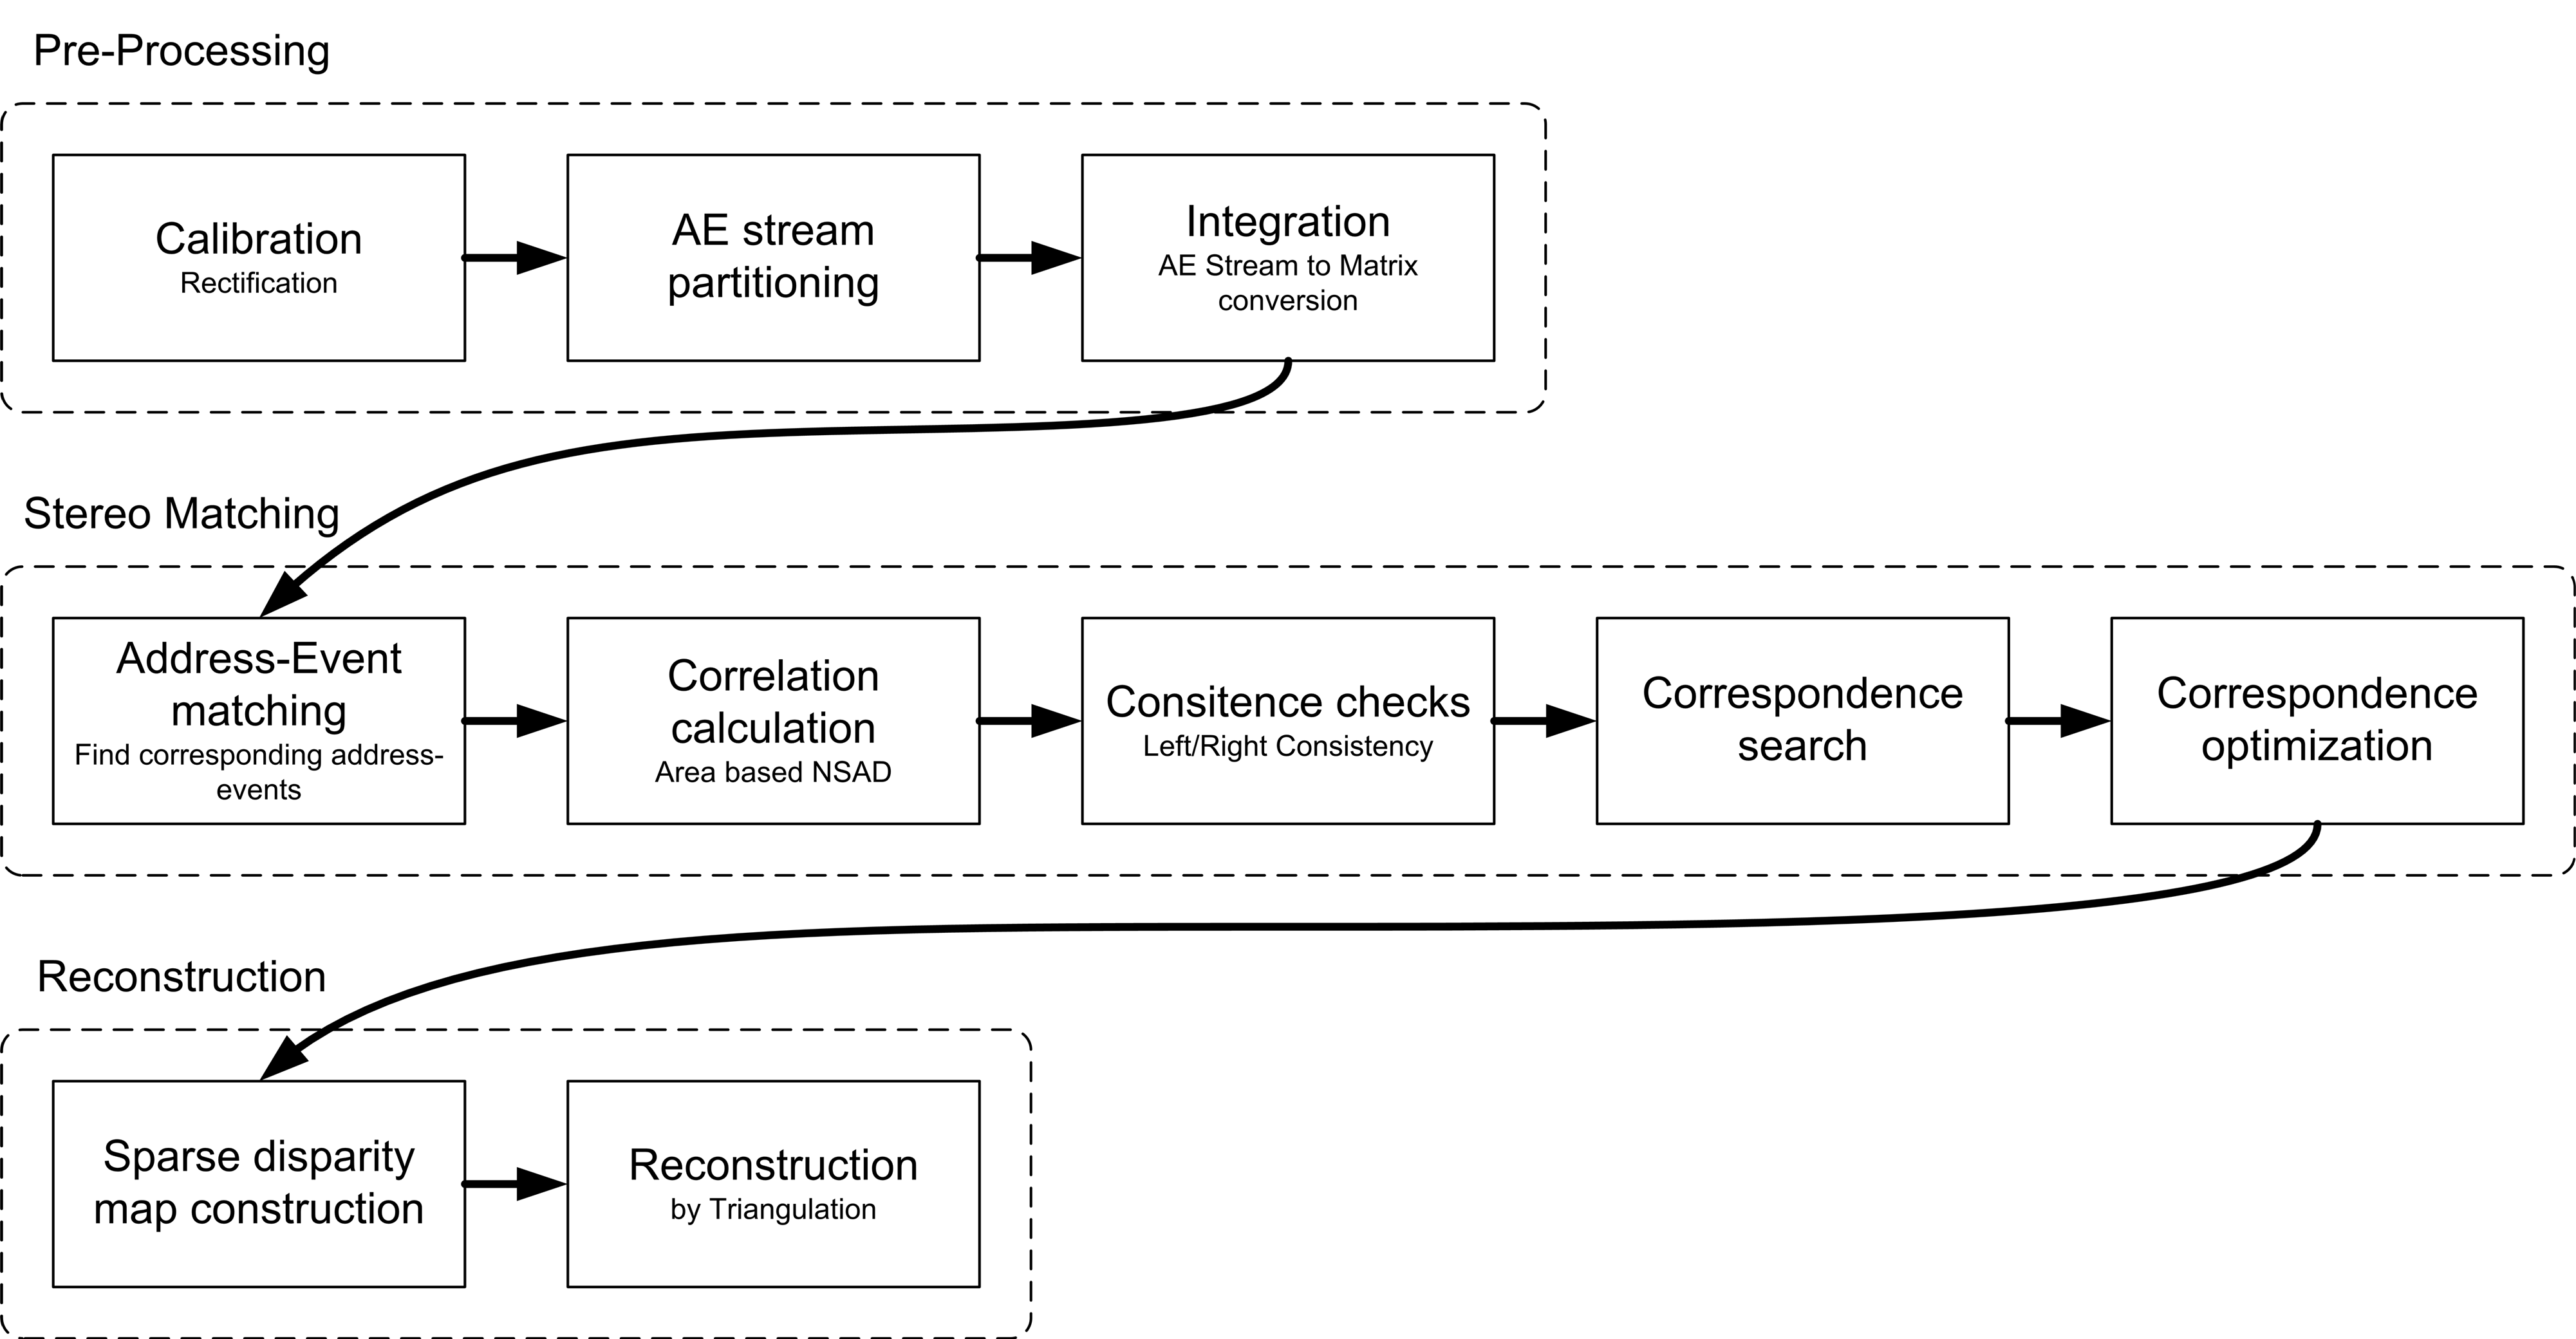
\includegraphics[height=60mm]{Images/DVS_stereo.png}
	\end{center}
	\caption{A block diagram that shows the stereo matching algorithm in \citet{Belbachir01}}
	\label{fig:DVS_stereo}
\end{figure}

In the stereo matching phase, potential matches are searched and the matching cost for all possibles matches is calculated. This is done from both sides to assure constistency. Actually matching events are found by minimizing the earlier calculated cost. 

The distance between matching pixels is put into a disparity map which shows all found events with corresponding distances. 

\section{Approach}
On the basis of DVS and the mentioned stereo matching algorithm, a system can be designed that enables efficient object tracking in three dimension with limited resources. Events can be extracted from a stream of images by comparing consecutive images and remembering pixel positions with changing intensity. The resulting events can be processed in the same way as describe above. A usual image sensor already delivers whole frames which means that there is no need for the stream partitioning step. The rest of the steps don't depend on the choice of the sensor. 

Research can be done for the correlation calculation block as there are several algorithms for this step with different characteristics. Consistency may or may not be necessary and there may exist less resource-intensive ways to ensure consistent results. 

In order to demonstrate the capabilities of the system, the disparity map can be used to track an object and measure its path. Accuracy of the path displays the effectiveness of the system while resource usage gives a measure of the efficiency of the designed system. 
\appendix
\chapter{Appendix 1} \label{app:one}
Tip: Make a copy of this document, since this is a manual of the template. This
will prevent losing the document while modifying it. (And probably breaking
it.)

\section{Required TexLive packages} 
The following packages are required for TeX Live 2012 and 2013 (tested under Ubuntu) 
\begin{verbatim} 
texlive
texlive-lang-dutch     -> Dutch hypenation
                          (old TeX Live distributions, 2013-)
texlive-lang-europeans -> Dutch hypenation (amongst others)
                          (new Tex Live distributions 2013+)
texlive-latex-extra
texlive-fonts-extra    -> fourier
texlive-humanities     -> lineno
texlive-pstricks       -> pstricks (2013+?)
                          (not really used in the template??)
\end{verbatim}


% Bibliography starts here
\backmatter

% Generate bibliography
\fancyhead[LO]{Bibliography}
\bibliographystyle{include/files/RaM-bibtex}
\label{ch:bib} %label to refer to
\bibliography{bibliography} 

\end{document}

